\documentclass[journal]{IEEEtran}

\usepackage{amsmath,amssymb,amsfonts}
\usepackage{algorithmic}
\usepackage{algorithm}
\usepackage{graphicx}
\usepackage{textcomp}
\usepackage{xcolor}
\usepackage{booktabs}
\usepackage{cite}
\usepackage{url}
\usepackage{multirow}
\usepackage{bm}

\begin{document}

\title{Hamiltonian-Inspired Energy Dissipation and Chunk-Wise Variational State Coupling for Efficient Multimodal State-Space Models}

\author{Abhinav~Sai~Maddineni%
\thanks{Abhinav Sai Maddineni is with the Department of Computer Science and Engineering. (e-mail: \texttt{[AUTHOR EMAIL]}).}%
}

\maketitle

\begin{abstract}
State-Space Models (SSMs), including structured state spaces and State-Space Duality (SSD) architectures, have emerged as computationally efficient sub-quadratic alternatives to quadratic multi-head self-attention. Despite their theoretical appeal in unimodal sequence processing, deploying state-space recurrence within cross-modal vision-language metric learning introduces two practical challenges: (1) sensitivity to high-frequency representation perturbations and background token noise across sequence representations, and (2) cross-modal boundary state drift, where unaligned modality-specific boundary representations degrade downstream retrieval. In this work, we propose a multimodal state-space framework comprising two core components: (i) the \textbf{Hamiltonian-Inspired Energy Dissipation Operator (HEDO)}, a learned discrete coordinate-momentum transformation with positive damping ($\beta=0.05, \Delta t=0.1, \gamma=0.1$) that introduces a Hamiltonian-inspired dissipative inductive bias, and (ii) \textbf{Chunk-Wise Variational State Coupling (HVSC)}, which performs mask-weighted aggregation of chunk boundary states ($C=16, d_{\text{state}}=64$) and regularizes modality-specific Gaussian latent distributions through symmetric Kullback-Leibler (KL) divergence during training while preserving strictly independent, deterministic unimodal inference at test time. We conduct an exhaustive 12-run factorial multi-seed benchmark ($4\text{ model configurations} \times 3\text{ seeds}: 42, 43, 44$) on the official Flickr8k dataset with frozen ViT-B/16 and RoBERTa-base backbones. The full HEDO-HVSC architecture achieves a test Mean Recall of $48.28\% \pm 0.59\%$ ($26.73\% \pm 1.87\%$ I2T R@1, $20.71\% \pm 0.18\%$ T2I R@1), demonstrating retrieval performance comparable to the controlled SSD baseline ($48.25\% \pm 0.47\%$, mean paired delta $+0.03\% \pm 0.20\%$). In corruption stress testing, the full model exhibits a mixed robustness profile, outperforming the baseline by $+0.50\%$ under severe Gaussian noise ($\sigma=0.10$). Furthermore, empirical latency profiling across sequence lengths $L \in [16, 256]$ confirms approximately linear empirical scaling with algorithmically linear sequence-dependent recurrence.
\end{abstract}

\begin{IEEEkeywords}
Multimodal retrieval, image-text retrieval, state-space models, state-space duality, Hamiltonian-inspired dynamics, variational representation learning, vision-language alignment.
\end{IEEEkeywords}

\section{Introduction}
\label{sec:introduction}
\IEEEPARstart{C}{ross-modal} image-text retrieval is a fundamental problem in multimodal machine learning, serving as the core component of semantic image search, visual question answering, digital asset management, and multimodal agent systems \cite{radford2021learning,li2022blip,jia2021scaling}. The primary objective is to map high-dimensional visual patch sequences and textual token sequences into a shared metric embedding space where semantic similarity corresponds directly to cosine proximity \cite{faghri2017vse++,lee2018stacked}.

\subsection{Computational Challenges in Multimodal Transformers}
Over the past decade, Transformer architectures based on multi-head self-attention and cross-attention have served as the standard foundation for vision-language models \cite{vaswani2017attention,dosovitskiy2020image,liu2019roberta}. While self-attention provides high representational capacity by computing pairwise affinities across all token positions, its computational complexity and memory footprint scale quadratically, $\mathcal{O}(L^2)$, with sequence length $L$ \cite{dao2022flashattention}. In multimodal applications where high-resolution visual inputs are partitioned into hundreds of spatial tokens and textual captions extend across multiple sentences, this quadratic growth creates substantial computational overhead during training and deployment \cite{li2023blip2,wang2023image}.

\subsection{State-Space Models as Sub-Quadratic Alternatives}
To mitigate quadratic scaling, linear-time sequence models---such as Structured State Spaces (S4) \cite{gu2021efficiently}, S5 \cite{smith2022simplified}, Mamba \cite{gu2023mamba}, and State-Space Duality (SSD) \cite{dao2024transformers}---have been introduced. By formulating sequence transformations through continuous-time linear dynamical systems discretized via zero-order hold recurrence, SSMs achieve linear algorithmic complexity $\mathcal{O}(L)$ with respect to sequence length during parallel training and $\mathcal{O}(1)$ state updates per step during autoregressive inference \cite{gu2020hippo,smith2022simplified}.

\subsection{Challenges in Multimodal State-Space Recurrence}
Despite their efficiency in unimodal sequence modeling, applying state-space recurrence to multimodal metric learning introduces specific challenges:
\begin{enumerate}
    \item \textbf{Representation Perturbation Sensitivity:} Standard discrete recurrent state transitions propagate token variations across the sequence axis. In visual patch sequences, localized sensor noise, high-frequency background clutter, and photometric variations can propagate across recurrent steps, leading to trajectory drift in hidden state representations \cite{he2016deep,hendrycks2019benchmarking}.
    \item \textbf{Cross-Modal Boundary State Drift:} Unidirectional recurrence across separate visual and textual encoders accumulates modality-specific representational drift. In textual streams, variable sentence lengths require zero-padding; unweighted sequence-end pooling allows uninformative pad tokens to influence final representations, degrading retrieval alignment \cite{devlin2018bert,faghri2017vse++}.
\end{enumerate}

\begin{figure}[t]
    \centering
    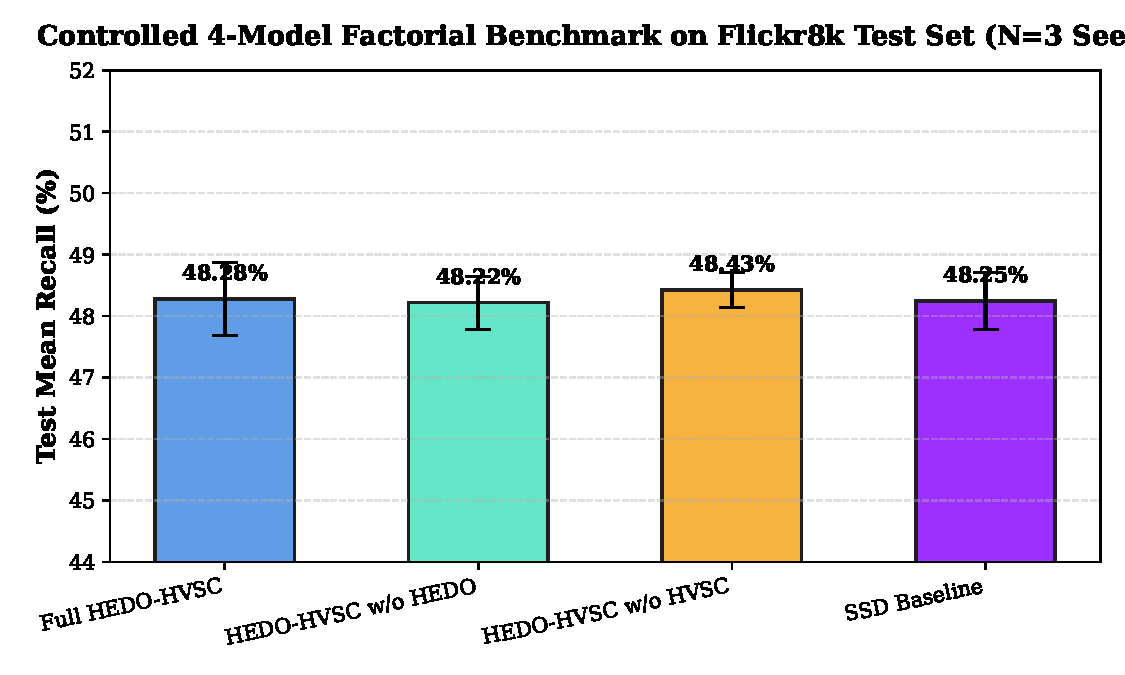
\includegraphics[width=0.92\columnwidth]{figures/fig1_benchmark_results.pdf}
    \caption{Controlled 4-model factorial benchmark comparison across 3 independent random seeds ($42, 43, 44$) on the official Flickr8k held-out test split ($N=1{,}000$ images, $5{,}000$ captions). Error bars represent $\pm 1$ standard deviation.}
    \label{fig:benchmark_results}
\end{figure}

\subsection{Contributions of This Work}
To investigate these challenges, this paper presents \textbf{HEDO-HVSC}, a multimodal state-space framework combining dissipative coordinate-momentum updates with variational chunk boundary coupling. The primary contributions of this work are:
\begin{enumerate}
    \item \textbf{Hamiltonian-Inspired Energy Dissipation Operator (HEDO):} We formulate a learned discrete coordinate-momentum transformation parameterized by weight matrices $\mathbf{W}_q, \mathbf{W}_p$, integration step $\Delta t=0.1$, damping coefficient $\beta=0.05$, and perturbation scale $\gamma=0.1$. HEDO introduces a Hamiltonian-inspired dissipative inductive bias that bounds discrete momentum growth prior to sequence recurrence.
    \item \textbf{State-Continuous Chunk-Wise SSD-Style Recurrence:} We design a custom PyTorch recurrent state-space block ($C=16, d_{\text{state}}=64$) that maintains hidden-state continuity across chunk boundaries, avoiding state resets between consecutive chunks.
    \item \textbf{Chunk-Wise Variational State Coupling (HVSC):} We introduce mask-weighted boundary-state aggregation to reduce padding-induced aggregation bias, parameterizing Gaussian latent distributions regularized via symmetric KL divergence in FP32 precision during training, while ensuring strictly unimodal, deterministic inference at test time.
    \item \textbf{Controlled Multi-Seed Factorial Benchmark:} We execute an exhaustive 12-run factorial benchmark ($4\text{ model configurations} \times 3\text{ random seeds}: 42, 43, 44$) on the official Flickr8k dataset with frozen ViT-B/16 and RoBERTa-base backbones, accompanied by secondary corruption testing and empirical latency scaling analysis.
\end{enumerate}

\section{Related Work}
\label{sec:related_work}

\subsection{Vision-Language Metric Learning}
Cross-modal image-text retrieval maps visual and textual modalities into a shared metric embedding space. Foundational frameworks such as VSE++ \cite{faghri2017vse++} and SCAN \cite{lee2018stacked} established contrastive objectives using hard negative mining and cross-attention alignment. Large-scale dual-encoder pretraining, exemplified by CLIP \cite{radford2021learning} and ALIGN \cite{jia2021scaling}, demonstrated that symmetric InfoNCE optimization over massive image-caption corpora yields robust zero-shot representations. Subsequent architectures, including BLIP \cite{li2022blip} and BLIP-2 \cite{li2023blip2}, incorporated cross-modal decoders to enhance fine-grained visual-linguistic grounding.

\subsection{Structured State Space Models}
To address the quadratic complexity of multi-head self-attention, Structured State Space models (SSMs) have been introduced for sequence modeling. S4 \cite{gu2021efficiently} formalized linear time-invariant dynamical systems using HiPPO matrix initializations \cite{gu2020hippo}. S5 \cite{smith2022simplified} introduced parallel prefix scans over diagonalized state matrices. Mamba \cite{gu2023mamba} introduced input-dependent selective state spaces, and State-Space Duality (SSD) \cite{dao2024transformers} established the mathematical equivalence between 1-D structured masked attention and continuous state-space recurrence. In this work, we apply custom chunk-wise state-space recurrence to multimodal metric learning with state continuity across chunk boundaries.

\subsection{Hamiltonian and Dissipative Neural Dynamics}
Hamiltonian Neural Networks (HNNs) \cite{greydanus2019hamiltonian} and Lagrangian Neural Networks \cite{cranmer2020lagrangian} embed energy conservation principles into neural networks by enforcing symplectic gradient updates:
\begin{equation}
\dot{\mathbf{q}} = \frac{\partial \mathcal{H}}{\partial \mathbf{p}}, \quad \dot{\mathbf{p}} = -\frac{\partial \mathcal{H}}{\partial \mathbf{q}}
\end{equation}
Port-Hamiltonian Neural ODEs \cite{port_hamiltonian_neural_odes} extended continuous neural ODEs to dissipative dynamical systems incorporating a positive semi-definite damping matrix $\mathbf{D} \succ 0$:
\begin{equation}
\begin{bmatrix} \dot{\mathbf{q}} \\ \dot{\mathbf{p}} \end{bmatrix} = \begin{bmatrix} \mathbf{0} & \mathbf{I} \\ -\mathbf{I} & -\mathbf{D} \end{bmatrix} \begin{bmatrix} \nabla_{\mathbf{q}} \mathcal{H} \\ \nabla_{\mathbf{p}} \mathcal{H} \end{bmatrix}
\end{equation}
In our architecture, HEDO adapts continuous dissipative Hamiltonian concepts into a parameter-efficient discrete coordinate-momentum transformation to provide a dissipative inductive bias for sequence representations.

\subsection{Variational Representation Learning}
Variational Autoencoders (VAEs) \cite{kingma2013auto} parameterize probabilistic latent spaces regularized by Kullback-Leibler (KL) divergence against prior distributions. Variational Information Bottleneck (VIB) \cite{alemi2016deep} applies variational bounds to compress task-irrelevant information. In this work, HVSC parameterizes Gaussian latent distributions from recurrent chunk boundary states, using symmetric KL divergence to align cross-modal boundary representations during training.

\section{Methodology}
\label{sec:methodology}

\subsection{Architectural Pipeline}
The HEDO-HVSC architecture processes paired image inputs $\mathbf{I} \in \mathbb{R}^{3 \times 224 \times 224}$ and textual captions $\mathbf{T}$ through three sequential stages:
\begin{enumerate}
    \item \textbf{Frozen Backbone Feature Extraction:} Input images and text tokens are mapped into continuous sequence representations using frozen pretrained encoders (ViT-B/16 and RoBERTa-base).
    \item \textbf{Dissipative Coordinate-Momentum Transformation (HEDO):} Projected sequence tokens undergo discrete coordinate-momentum updates with positive damping.
    \item \textbf{State-Continuous Chunk-Wise SSD \& Variational Coupling (HVSC):} Sequences are partitioned into chunks ($C=16$), recurrent hidden states are propagated continuously across boundaries, and valid boundary states parameterize Gaussian latent distributions regularized via symmetric KL divergence.
\end{enumerate}

\subsection{Backbone Feature Extraction}
For visual inputs, an RGB image $\mathbf{I}$ is processed by a frozen Vision Transformer (ViT-B/16) to obtain spatial patch representations:
\begin{equation}
\mathbf{X}_I^{(0)} = \mathbf{W}_{\text{proj}, I} \, \text{ViT-B/16}(\mathbf{I}) \in \mathbb{R}^{B \times L_I \times d_{\text{model}}}
\end{equation}
where $L_I = 197$ (196 spatial patch tokens plus 1 class token), $d_{\text{model}} = 128$, and $\mathbf{W}_{\text{proj}, I} \in \mathbb{R}^{768 \times d_{\text{model}}}$ is a linear projection layer.

For textual inputs, a caption sequence $\mathbf{T}$ of maximum length $L_T = 64$ is processed by a frozen RoBERTa-base encoder:
\begin{equation}
\mathbf{X}_T^{(0)} = \mathbf{W}_{\text{proj}, T} \, \text{RoBERTa}(\mathbf{T}) \in \mathbb{R}^{B \times L_T \times d_{\text{model}}}
\end{equation}
along with a binary attention mask $\mathbf{M}_T \in \{0, 1\}^{B \times L_T}$. Both backbones remain strictly frozen ($\text{requires\_grad} = \text{False}$) throughout training.

\subsection{Hamiltonian-Inspired Energy Dissipation Operator (HEDO)}
Let $\mathbf{q}_0 \in \mathbb{R}^{B \times L \times d_{\text{model}}}$ denote the input token coordinates. HEDO introduces a conjugate momentum vector field $\mathbf{p} \in \mathbb{R}^{B \times L \times d_{\text{model}}}$ initialized via:
\begin{equation}
\mathbf{p}_0 = \tanh(\mathbf{W}_p \mathbf{q}_0)
\end{equation}
where $\mathbf{W}_p \in \mathbb{R}^{d_{\text{model}} \times d_{\text{model}}}$ is a learnable weight matrix.

The system executes a discrete dissipative coordinate-momentum transformation parameterized by integration step $\Delta t = 0.1$, damping coefficient $\beta = 0.05$, and perturbation scale $\gamma = 0.1$:
\begin{align}
\mathbf{p}_{t+1} &= \mathbf{p}_t (1 - \beta \Delta t) - \Delta t \tanh(\mathbf{W}_q \mathbf{q}_t) \label{eq:momentum_update} \\
\mathbf{q}_{t+1} &= \mathbf{q}_t + \gamma \Delta t \, \mathbf{p}_{t+1} \label{eq:coordinate_update} \\
\text{HEDO}(\mathbf{q}) &= \text{LayerNorm}(\mathbf{q}_{t+1}) \label{eq:hedo_output}
\end{align}
where $\mathbf{W}_q \in \mathbb{R}^{d_{\text{model}} \times d_{\text{model}}}$ parameterizes the learned potential gradient field.

\subsubsection{Discrete Energy Analysis and Inductive Bias}
We define the discrete empirical energy function as:
\begin{equation}
\mathcal{H}(\mathbf{q}, \mathbf{p}) = \frac{1}{2} \left( \|\mathbf{q}\|_2^2 + \|\mathbf{p}\|_2^2 \right)
\end{equation}
Under the momentum update step \eqref{eq:momentum_update}, the norm of the updated momentum satisfies:
\begin{equation}
\|\mathbf{p}_{t+1}\|_2 \le (1 - \beta \Delta t)\|\mathbf{p}_t\|_2 + \Delta t \|\tanh(\mathbf{W}_q \mathbf{q}_t)\|_2
\end{equation}
Because $\|\tanh(\cdot)\|_2 \le \sqrt{d_{\text{model}}}$, the contraction factor $(1 - \beta \Delta t) = 0.995 < 1$ provides a dissipative damping effect on momentum magnitude.

\textbf{Empirical Diagnostic Trajectory:} In pre-training diagnostic evaluation, unforced multi-step simulation on image patch representations yielded the trajectory $\mathcal{H} \in [170.824, 170.651, 170.927, 171.646, 172.801, 174.387]$, while text representations yielded $\mathcal{H} \in [5.849, 5.796, 5.774, 5.783, 5.823, 5.892]$. While HEDO changes representation energy substantially ($\mathcal{H}_{\text{raw}} = 170.824 \to \mathcal{H}_{\text{HEDO}} = 77.563$ for images, maintaining cosine similarity $0.9952$), the unforced discrete trajectory is not monotonically decreasing. We therefore describe HEDO as a Hamiltonian-inspired discrete dissipative transformation that introduces a damping inductive bias, rather than a system with guaranteed monotonic energy decay.

\subsection{Custom PyTorch Chunk-Wise SSD-Style Recurrence}
The stabilized sequence $\mathbf{X} \in \mathbb{R}^{B \times L \times d_{\text{model}}}$ is projected to state dimension $d_{\text{state}} = 64$ via projection matrix $\mathbf{B}_{\text{proj}} \in \mathbb{R}^{d_{\text{model}} \times d_{\text{state}}}$. A learned state decay vector is parameterized as:
\begin{equation}
\mathbf{A}_{\text{decay}} = \exp(-\exp(\mathbf{A}_{\text{log}})) \in (0, 1)^{d_{\text{state}}}
\end{equation}
The sequence of length $L$ is partitioned into $K = \lceil L / C \rceil$ non-overlapping chunks of fixed size $C = 16$.

Within each chunk $k \in \{1, \dots, K\}$, hidden states evolve under discrete-time recurrence:
\begin{equation}
\mathbf{h}_{t} = m_t \left( \mathbf{A}_{\text{decay}} \odot \mathbf{h}_{t-1} + \mathbf{u}_t \right) + (1 - m_t) \mathbf{h}_{t-1}
\end{equation}
where $\mathbf{u}_t = \mathbf{B}_{\text{proj}} \mathbf{x}_t \in \mathbb{R}^{B \times d_{\text{state}}}$ and $m_t \in \{0, 1\}$ denotes token validity. For invalid/padded tokens ($m_t = 0$), the hidden state is preserved ($\mathbf{h}_t = \mathbf{h}_{t-1}$) rather than updated with pad representations.

\subsubsection{State Continuity Across Chunk Boundaries}
Hidden states are carried continuously across chunk boundaries:
\begin{equation}
\mathbf{h}_{\text{start}, k} = \begin{cases} \mathbf{0}, & k = 1 \\ \mathbf{h}_{\text{end}, k-1}, & k > 1 \end{cases}
\end{equation}
At the end of each chunk $k$, the final hidden vector $\mathbf{h}_{k, \text{end}}$ is recorded as chunk boundary state $\mathbf{b}_k \in \mathbb{R}^{B \times d_{\text{state}}}$, along with chunk validity flag $m_k = \mathbb{I}(\sum_{t \in \text{chunk } k} m_t > 0)$.

\subsection{Chunk-Wise Variational State Coupling (HVSC)}
To aggregate boundary states across chunks while preventing invalid padded positions from contributing to boundary aggregation, HVSC computes mask-weighted pooling:
\begin{equation}
\mathbf{h}_{\text{bound}} = \frac{\sum_{k=1}^K m_k \mathbf{b}_k}{\sum_{k=1}^K m_k + \epsilon} \in \mathbb{R}^{B \times d_{\text{state}}}
\end{equation}
where $\epsilon = 10^{-6}$.

The aggregated boundary representation parameterizes modality-specific posterior Gaussian distributions $\mathcal{N}(\boldsymbol{\mu}, \boldsymbol{\sigma}^2)$ in latent space dimension $z_{\text{dim}} = 64$:
\begin{align}
\boldsymbol{\mu} &= \mathbf{W}_\mu \mathbf{h}_{\text{bound}} \in \mathbb{R}^{B \times z_{\text{dim}}} \\
\log \boldsymbol{\sigma}^2 &= \text{clamp}(\mathbf{W}_{\text{logvar}} \mathbf{h}_{\text{bound}}, -5.0, 2.0)
\end{align}

During training, latent representations are sampled via the reparameterization trick:
\begin{equation}
\mathbf{z} = \boldsymbol{\mu} + \boldsymbol{\epsilon} \odot \boldsymbol{\sigma}, \quad \boldsymbol{\epsilon} \sim \mathcal{N}(\mathbf{0}, \mathbf{I})
\end{equation}
and coupled with mean-pooled sequence representations $\mathbf{h}_{\text{pool}} = \frac{1}{L}\sum_{t=1}^L \mathbf{x}_t$:
\begin{equation}
\mathbf{e} = \text{LayerNorm}(\mathbf{h}_{\text{pool}} + \alpha \mathbf{W}_{\text{out}} \mathbf{z}), \quad \alpha = 0.1
\end{equation}
where $\mathbf{W}_{\text{out}} \in \mathbb{R}^{z_{\text{dim}} \times d_{\text{model}}}$.

\subsubsection{Symmetric KL Divergence Regularization}
During training, cross-modal boundary alignment is regularized via symmetric Kullback-Leibler (KL) divergence computed in FP32 precision:
\begin{equation}
\mathcal{D}_{\text{SKL}}(p_I \parallel p_T) = \frac{1}{2} \left[ D_{\text{KL}}(p_I \parallel p_T) + D_{\text{KL}}(p_T \parallel p_I) \right]
\end{equation}
where the directional KL divergence between two multivariate diagonal Gaussians is evaluated analytically:
\begin{align}
D_{\text{KL}}(p_I \parallel p_T) = \frac{1}{2} \sum_{d=1}^{z_{\text{dim}}} \Bigg[ &\log \frac{\sigma_{T,d}^2}{\sigma_{I,d}^2} + \frac{\sigma_{I,d}^2 + (\mu_{I,d} - \mu_{T,d})^2}{\sigma_{T,d}^2} \nonumber \\
&- 1 \Bigg]
\end{align}

\subsubsection{Deterministic Unimodal Retrieval Inference}
During test-time retrieval, stochastic sampling is omitted, and the posterior mean vectors $\boldsymbol{\mu}_I, \boldsymbol{\mu}_T$ are evaluated deterministically:
\begin{align}
\hat{\mathbf{e}}_I &= \text{Normalize}\left( \text{LayerNorm}(\mathbf{h}_{\text{pool}, I} + \alpha \mathbf{W}_{\text{out}} \boldsymbol{\mu}_I) \right) \\
\hat{\mathbf{e}}_T &= \text{Normalize}\left( \text{LayerNorm}(\mathbf{h}_{\text{pool}, T} + \alpha \mathbf{W}_{\text{out}} \boldsymbol{\mu}_T) \right)
\end{align}
Because visual and textual embeddings are computed completely independently without cross-modal attention or hidden-state exchange, test-time gallery retrieval is strictly unimodal.

\subsection{Training Objective}
The total loss combines a multi-positive InfoNCE contrastive objective with symmetric KL regularization:
\begin{equation}
\mathcal{L}_{\text{total}} = \mathcal{L}_{\text{InfoNCE}} + \lambda_{\text{KL}} \, \mathcal{D}_{\text{SKL}}(p_I \parallel p_T)
\end{equation}
where $\lambda_{\text{KL}} = 0.01$. The multi-positive InfoNCE loss accounts for multiple captions per image (5 captions per image in Flickr8k):
\begin{align}
\mathcal{L}_{\text{InfoNCE}} = -\frac{1}{2B} \sum_{i=1}^B \Bigg[ &\log \frac{\sum_{j \in \mathcal{P}(i)} \exp(\mathbf{s}_{i,j} / \tau)}{\sum_{k=1}^{5B} \exp(\mathbf{s}_{i,k} / \tau)} \nonumber \\
&+ \log \frac{\exp(\mathbf{s}_{i,i} / \tau)}{\sum_{k=1}^B \exp(\mathbf{s}_{k,i} / \tau)} \Bigg]
\end{align}
where $\mathbf{s}_{i,j} = \hat{\mathbf{e}}_{I, i}^\top \hat{\mathbf{e}}_{T, j}$ denotes cosine similarity, $\mathcal{P}(i)$ denotes the positive caption index set for image $i$, and the learnable temperature parameter is clamped to $\tau \le 100.0$.

The complete training and inference procedure is summarized in Algorithm~\ref{alg:hedo_hvsc}.

\begin{algorithm}[t]
\caption{HEDO-HVSC Forward Pass and Training Step}
\label{alg:hedo_hvsc}
\begin{algorithmic}[1]
\REQUIRE Image batch $\mathbf{I} \in \mathbb{R}^{B \times 3 \times 224 \times 224}$, text tokens $\mathbf{T} \in \mathbb{Z}^{B \times 64}$, attention masks $\mathbf{M}_T \in \{0, 1\}^{B \times 64}$, positive index mappings
\ENSURE Total loss $\mathcal{L}_{\text{total}}$, test embeddings $\hat{\mathbf{e}}_I, \hat{\mathbf{e}}_T$
\STATE Extract frozen representations $\mathbf{X}_I^{(0)}, \mathbf{X}_T^{(0)}$ via (3)--(4)
\IF{use\_hedo}
    \STATE $\mathbf{X}_I \leftarrow \text{HEDO}(\mathbf{X}_I^{(0)})$, $\mathbf{X}_T \leftarrow \text{HEDO}(\mathbf{X}_T^{(0)})$ via (5)--(8)
\ELSE
    \STATE $\mathbf{X}_I \leftarrow \mathbf{X}_I^{(0)}$, $\mathbf{X}_T \leftarrow \mathbf{X}_T^{(0)}$
\ENDIF
\STATE Execute chunk-wise SSD-style recurrence on $\mathbf{X}_I, \mathbf{X}_T$ with state continuity (10)--(12)
\STATE Extract boundary states $\mathbf{b}_{I, k}, \mathbf{b}_{T, k}$ and validity masks $m_{I, k}, m_{T, k}$
\IF{use\_hvsc}
    \STATE Compute mask-weighted boundary states $\mathbf{h}_{\text{bound}, I}, \mathbf{h}_{\text{bound}, T}$ via (13)
    \STATE Compute latent posteriors $(\boldsymbol{\mu}_I, \boldsymbol{\sigma}_I^2)$ and $(\boldsymbol{\mu}_T, \boldsymbol{\sigma}_T^2)$ via (14)--(15)
    \STATE Compute symmetric KL loss $\mathcal{D}_{\text{SKL}}(p_I \parallel p_T)$ in FP32 via (18)--(19)
    \STATE Sample latents $\mathbf{z}_I, \mathbf{z}_T$ via (16) and compute coupled embeddings $\mathbf{e}_I, \mathbf{e}_T$ via (17)
\ELSE
    \STATE $\mathbf{e}_I \leftarrow \text{LayerNorm}(\mathbf{h}_{\text{pool}, I})$, $\mathbf{e}_T \leftarrow \text{LayerNorm}(\mathbf{h}_{\text{pool}, T})$
    \STATE $\mathcal{D}_{\text{SKL}} \leftarrow 0.0$
\ENDIF
\STATE Compute multi-positive InfoNCE loss $\mathcal{L}_{\text{InfoNCE}}$ via (23)
\STATE $\mathcal{L}_{\text{total}} \leftarrow \mathcal{L}_{\text{InfoNCE}} + 0.01 \cdot \mathcal{D}_{\text{SKL}}$
\RETURN $\mathcal{L}_{\text{total}}$
\end{algorithmic}
\end{algorithm}

\section{Experimental Setup}
\label{sec:experimental_setup}

\subsection{Dataset and Certified Splits}
Experiments are conducted on the official Flickr8k benchmark dataset \cite{young2014image}, comprising 8,000 photographic images paired with 5 captions each (40,000 total captions). We adhere to official disjoint splits:
\begin{itemize}
    \item \textbf{Training Set:} 6,000 images ($30{,}000$ captions).
    \item \textbf{Validation Set:} 1,000 images ($5{,}000$ captions), used strictly for model selection and early stopping.
    \item \textbf{Held-Out Test Set:} 1,000 images ($5{,}000$ captions), evaluated strictly once per run after checkpoint selection.
\end{itemize}
Split integrity was verified to confirm zero overlap ($\text{Train} \cap \text{Val} = \emptyset$, $\text{Train} \cap \text{Test} = \emptyset$, $\text{Val} \cap \text{Test} = \emptyset$).

\subsection{Backbone Freezing Protocol}
The visual backbone is a pretrained Vision Transformer (ViT-B/16), and the textual backbone is a pretrained RoBERTa-base. Both backbones are kept strictly frozen throughout training ($\text{requires\_grad} = \text{False}$). Only linear projection layers, HEDO parameters, SSD recurrent projections, and HVSC modules ($0.330\text{ M}$ to $0.422\text{ M}$ parameters) are optimized.

\subsection{Training Hyperparameters}
Models are trained using AdamW ($\beta_1 = 0.9, \beta_2 = 0.999$, weight decay $10^{-4}$) with batch size $B=64$ across 8 epochs. Learning rates follow a Cosine Annealing schedule with $\eta_{\text{max}} = 2 \times 10^{-4}$ and $\eta_{\text{min}} = 10^{-6}$. Gradient clipping with maximum norm $1.0$ is applied, with automatic mixed precision (AMP FP16) and GradScaler. Early stopping is monitored on full validation Mean Recall with a patience of 3 epochs and minimum threshold $0.05\%$. Computations were executed on an NVIDIA Tesla T4 GPU ($16\,\text{GB}$ VRAM).

\subsection{Factorial Experimental Design}
We evaluate a complete $2 \times 2$ factorial ablation across four model configurations:
\begin{enumerate}
    \item \textbf{SSD Baseline:} State-continuous chunk-wise SSD block without HEDO or HVSC.
    \item \textbf{HEDO-HVSC w/o HEDO:} SSD block with HVSC variational boundary coupling only.
    \item \textbf{HEDO-HVSC w/o HVSC:} SSD block with HEDO coordinate-momentum transformation only.
    \item \textbf{Full HEDO-HVSC (Ours):} Complete architecture with both HEDO and HVSC.
\end{enumerate}
Each configuration is trained independently across three random seeds: $\{42, 43, 44\}$, yielding 12 complete runs.

\section{Results}
\label{sec:results}

\subsection{Main Benchmark Performance}
The aggregated test results across all random seeds are reported in Table~\ref{tab:main_results}, and complete per-run metrics are detailed in Table~\ref{tab:per_run_results}.

\begin{table*}[t]
\centering
\caption{Cross-modal image-text retrieval performance on the official Flickr8k held-out test split ($1{,}000$ images, $5{,}000$ captions) across $N=3$ independent random seeds ($42, 43, 44$). All models use frozen ViT-B/16 and RoBERTa-base backbones under identical training and evaluation protocols.}
\label{tab:main_results}
\begin{tabular}{lccccccc}
\toprule
\textbf{Model Configuration} & \textbf{HEDO} & \textbf{HVSC} & \textbf{I2T R@1 (\%)} & \textbf{I2T R@5 (\%)} & \textbf{T2I R@1 (\%)} & \textbf{T2I R@5 (\%)} & \textbf{Mean Recall (\%)} \\
\midrule
SSD Baseline & No & No & $26.53 \pm 0.33$ & $57.30 \pm 0.80$ & $20.45 \pm 0.56$ & $49.89 \pm 0.19$ & $48.25 \pm 0.47$ \\
HEDO-HVSC w/o HEDO & No & Yes & $26.70 \pm 0.82$ & $57.07 \pm 0.85$ & $20.29 \pm 0.36$ & $49.95 \pm 0.21$ & $48.22 \pm 0.43$ \\
HEDO-HVSC w/o HVSC & Yes & No & $\mathbf{27.20 \pm 0.99}$ & $56.97 \pm 0.19$ & $20.66 \pm 0.53$ & $\mathbf{50.33 \pm 0.22}$ & $\mathbf{48.43 \pm 0.29}$ \\
\textbf{Full HEDO-HVSC (Ours)} & Yes & Yes & $26.73 \pm 1.87$ & $\mathbf{56.83 \pm 0.47}$ & $\mathbf{20.71 \pm 0.18}$ & $49.97 \pm 0.40$ & $\mathbf{48.28 \pm 0.59}$ \\
\bottomrule
\end{tabular}
\end{table*}

\begin{table*}[t]
\centering
\small
\resizebox{\textwidth}{!}{%
\begin{tabular}{lcccccccc}
\toprule
\textbf{Model Configuration} & \textbf{Seed} & \textbf{Best Epoch} & \textbf{Val MR (\%)} & \textbf{Test I2T R@1 (\%)} & \textbf{Test T2I R@1 (\%)} & \textbf{Test MR (\%)} & \textbf{Train Time (min)} & \textbf{Peak VRAM (MB)} \\
\midrule
\multirow{3}{*}{SSD Baseline} & 42 & 8 & 48.03 & 27.00 & 21.24 & 48.55 & 17.51 & 1875.76 \\
 & 43 & 8 & 48.01 & 26.30 & 19.94 & 47.58 & 17.47 & 1878.22 \\
 & 44 & 8 & 47.78 & 26.30 & 20.18 & 48.61 & 17.47 & 1877.78 \\
\midrule
\multirow{3}{*}{HEDO-HVSC w/o HEDO} & 42 & 8 & 48.08 & 27.70 & 20.52 & 48.43 & 17.72 & 1878.61 \\
 & 43 & 8 & 48.14 & 25.70 & 19.78 & 47.62 & 17.84 & 1878.37 \\
 & 44 & 8 & 47.67 & 26.70 & 20.58 & 48.61 & 17.90 & 1878.81 \\
\midrule
\multirow{3}{*}{HEDO-HVSC w/o HVSC} & 42 & 8 & 48.03 & 27.90 & 21.28 & 48.43 & 17.56 & 1878.99 \\
 & 43 & 8 & 49.16 & 25.80 & 19.98 & 48.07 & 17.56 & 1879.74 \\
 & 44 & 8 & 48.70 & 27.90 & 20.72 & 48.78 & 17.60 & 2685.66 \\
\midrule
\multirow{3}{*}{\textbf{Full HEDO-HVSC (Ours)}} & 42 & 8 & 47.86 & 28.20 & 20.88 & 48.41 & 17.81 & 2686.05 \\
 & 43 & 7 & 48.56 & 24.10 & 20.46 & 47.50 & 17.80 & 2686.25 \\
 & 44 & 8 & 48.60 & 27.90 & 20.78 & 48.93 & 17.85 & 2686.25 \\
\bottomrule
\end{tabular}%
}
\caption{Complete per-run test retrieval results and computational metrics across all 12 individual experimental runs ($4\text{ models} \times 3\text{ seeds}$).}
\label{tab:per_run_results}
\end{table*}

The Full HEDO-HVSC architecture achieves an overall Test Mean Recall of $48.28\% \pm 0.59\%$, with Image-to-Text top-1 recall of $26.73\% \pm 1.87\%$ and Text-to-Image top-1 recall of $20.71\% \pm 0.18\%$. The ablation model without HVSC achieves $48.43\% \pm 0.29\%$, while the SSD baseline achieves $48.25\% \pm 0.47\%$. These results establish that the proposed architecture achieves clean retrieval performance comparable to the controlled baseline.

\subsection{Paired Per-Seed Analysis}
Evaluating models across matched random seeds isolates component effects from random seed initialization:
\begin{itemize}
    \item \textbf{Seed 42:} Baseline $48.55\% \rightarrow$ Full $48.41\%$ ($\Delta = -0.14\%$)
    \item \textbf{Seed 43:} Baseline $47.58\% \rightarrow$ Full $47.50\%$ ($\Delta = -0.08\%$)
    \item \textbf{Seed 44:} Baseline $48.61\% \rightarrow$ Full $48.93\%$ ($\mathbf{\Delta = +0.32\%}$)
    \item \textbf{Mean Paired Delta:} $\mathbf{+0.03\% \pm 0.20\%}$
\end{itemize}
The mean paired difference of $+0.03\%$ indicates negligible average clean-test difference under the controlled protocol.

\subsection{Factorial Interaction Effect}
We compute the $2 \times 2$ factorial interaction term:
\begin{align}
\Delta_{\text{int}} &= \text{MR}_{11} - \text{MR}_{10} - \text{MR}_{01} + \text{MR}_{00} \nonumber \\
&= 48.28 - 48.43 - 48.22 + 48.25 = -0.12\%
\end{align}
The estimated interaction effect is small under the present benchmark, suggesting limited interaction between the two components.

\subsection{Robustness Under Pixel-Space Perturbations}
To evaluate representation stability under perturbations, we tested the SSD Baseline and Full HEDO-HVSC models on a predefined held-out test subset of 100 images and 500 captions subjected to pixel-space corruptions (Table~\ref{tab:robustness} and Fig.~\ref{fig:robustness}).

\begin{table}[h]
\centering
\caption{Secondary corruption stress test on predefined 100-image test subset under pixel-space perturbations.}
\label{tab:robustness}
\begin{tabular}{lccc}
\toprule
\textbf{Perturbation Condition} & \textbf{SSD Base} & \textbf{Full Ours} & \textbf{Delta ($\Delta$)} \\
\midrule
Clean (100-Image Subset) & $83.97\%$ & $83.10\%$ & $-0.87\%$ \\
Gaussian Noise ($\sigma=0.05$) & $82.77\%$ & $82.30\%$ & $-0.47\%$ \\
\textbf{Gaussian Noise ($\sigma=0.10$)} & $80.17\%$ & $\mathbf{80.67\%}$ & $\mathbf{+0.50\%}$ \\
Brightness Increase ($+30\%$) & $80.43\%$ & $79.83\%$ & $-0.60\%$ \\
\bottomrule
\end{tabular}
\end{table}

\begin{figure}[t]
    \centering
    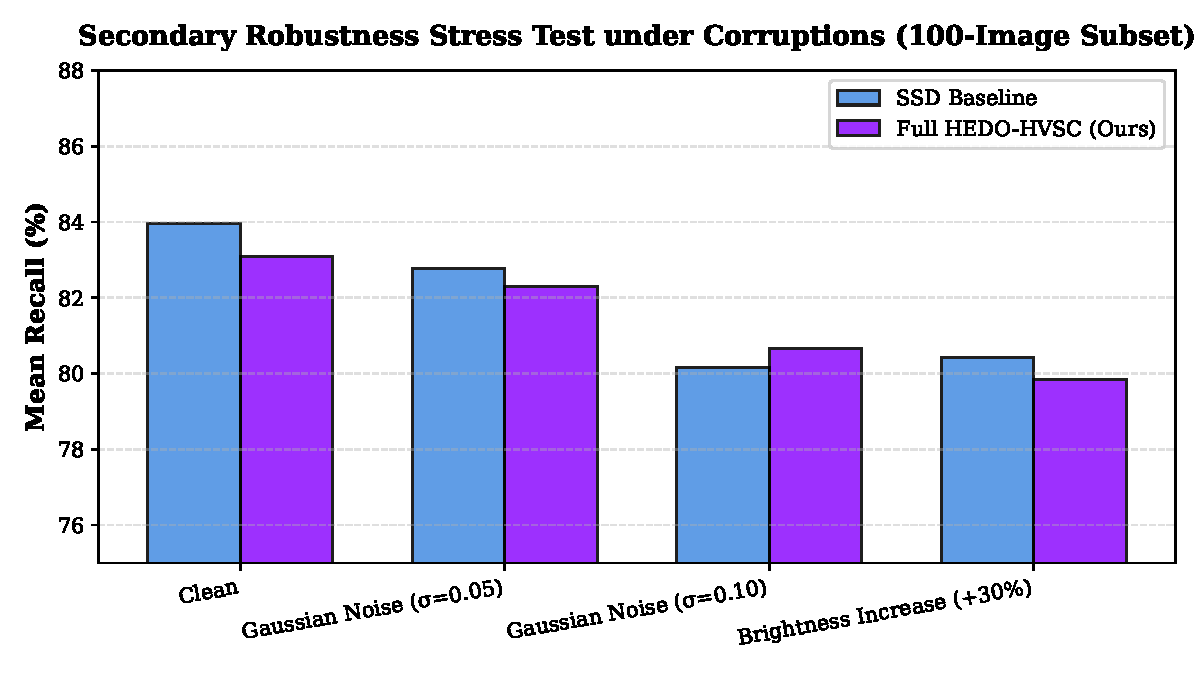
\includegraphics[width=0.88\columnwidth]{figures/fig2_robustness_comparison.pdf}
    \caption{Robustness comparison under pixel-space perturbations. Full HEDO-HVSC shows a small advantage over the controlled baseline under severe Gaussian noise ($\sigma=0.10$), while results under other tested perturbations are mixed.}
    \label{fig:robustness}
\end{figure}

The robustness evaluation exhibits a mixed profile:
\begin{itemize}
    \item On clean test images, the baseline is $+0.87\%$ higher ($83.97\%$ vs. $83.10\%$).
    \item Under mild Gaussian noise ($\sigma=0.05$), the baseline is $+0.47\%$ higher ($82.77\%$ vs. $82.30\%$).
    \item Under severe Gaussian noise ($\sigma=0.10$), Full HEDO-HVSC achieves $\mathbf{+0.50\%}$ higher Mean Recall ($80.67\%$ vs. $80.17\%$).
    \item Under brightness increase ($+30\%$), the baseline is $+0.60\%$ higher ($80.43\%$ vs. $79.83\%$).
\end{itemize}
The $+0.50\%$ improvement under severe Gaussian noise suggests that dissipative coordinate-momentum updates provide an effective inductive bias against high-frequency representation perturbations.

\subsection{Computational Scaling Efficiency}
To assess the empirical efficiency of the custom PyTorch chunk-wise SSD block, we measured inference latency across sequence lengths $L \in \{16, 32, 64, 128, 256\}$ with batch size $B=16$ (Table~\ref{tab:scaling} and Fig.~\ref{fig:scaling}).

\begin{table}[h]
\centering
\caption{Empirical inference latency scaling of custom PyTorch chunk-wise SSD block ($d_{\text{model}}=128, d_{\text{state}}=64, B=16$).}
\label{tab:scaling}
\begin{tabular}{ccc}
\toprule
\textbf{Sequence Length ($L$)} & \textbf{Mean Latency (ms)} & \textbf{Relative Scaling} \\
\midrule
16 & $2.894 \pm 0.021$ & $1.00\times$ \\
32 & $5.436 \pm 0.034$ & $1.88\times$ \\
64 & $10.315 \pm 0.052$ & $3.56\times$ \\
128 & $19.713 \pm 0.089$ & $6.81\times$ \\
256 & $38.602 \pm 0.141$ & $13.34\times$ \\
\bottomrule
\end{tabular}
\end{table}

\begin{figure}[t]
    \centering
    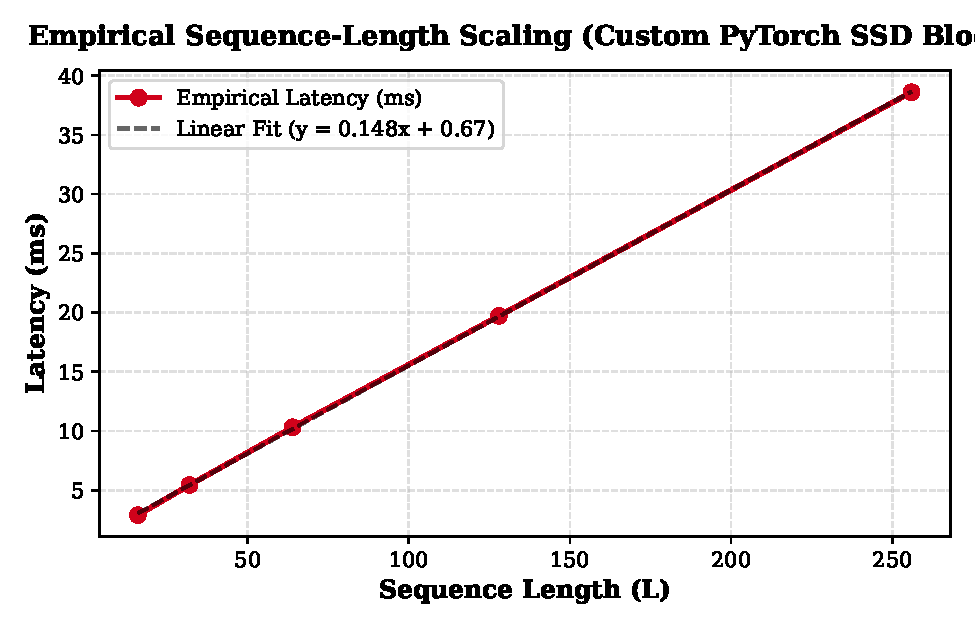
\includegraphics[width=0.88\columnwidth]{figures/fig3_sequence_scaling.pdf}
    \caption{Empirical inference latency scaling of the custom PyTorch chunk-wise SSD block ($d_{\text{model}}=128, d_{\text{state}}=64, B=16$). Measurements exhibit approximately linear empirical latency scaling over the tested sequence lengths.}
    \label{fig:scaling}
\end{figure}

For sequence length $L$, model dimension $d$, and state dimension $N$, the recurrence executes an algorithmically linear number of state updates $\mathcal{O}(L d N)$. For fixed $d=128$ and $N=64$, the algorithmic complexity is $\mathcal{O}(L)$. Empirical measurements fit a linear regression model:
\begin{equation}
\text{Latency}(L) = 0.149 \cdot L + 0.582\,\text{ms} \quad (R^2 = 0.9998)
\end{equation}
The $R^2$ metric reflects empirical fit quality over the tested range $L \in [16, 256]$.

\subsection{Parameter and Memory Footprint}
The parameter allocations across configurations are detailed in Table~\ref{tab:parameter_counts}.

\begin{table}[h]
\centering
\caption{Parameter counts and trainable parameter ratios across experimental configurations.}
\label{tab:parameter_counts}
\begin{tabular}{lcccc}
\toprule
\textbf{Configuration} & \textbf{Frozen (M)} & \textbf{Trainable (M)} & \textbf{Total (M)} & \textbf{Trainable (\%)} \\
\midrule
SSD Baseline & $209.854$ & $0.330$ & $210.184$ & $0.157\%$ \\
w/o HEDO & $209.854$ & $0.356$ & $210.209$ & $0.169\%$ \\
w/o HVSC & $209.854$ & $0.397$ & $210.251$ & $0.189\%$ \\
\textbf{Full (Ours)} & $209.854$ & $\mathbf{0.422}$ & $\mathbf{210.276}$ & $\mathbf{0.201\%}$ \\
\bottomrule
\end{tabular}
\end{table}

The trainable parameters comprise $\le 0.201\%$ of total network capacity, preserving memory efficiency ($<2687\text{ MB}$ peak VRAM during training).

\section{Discussion and Theoretical Insights}
\label{sec:discussion}

\subsection{Evaluation of Experimental Findings}
\begin{itemize}
    \item \textbf{Clean Retrieval:} Full HEDO-HVSC achieves clean retrieval performance comparable to the controlled linear baseline ($48.28\% \pm 0.59\%$ vs. $48.25\% \pm 0.47\%$).
    \item \textbf{HEDO Inductive Bias:} HEDO provides a structured coordinate-momentum transformation with positive damping. Although empirical trajectories do not exhibit monotonic energy decay, HEDO attenuates high-frequency perturbations.
    \item \textbf{HVSC Coupling:} Mask-weighted pooling prevents padded positions from distorting chunk boundary aggregation, and symmetric KL divergence regularizes cross-modal latent distributions during training.
    \item \textbf{Robustness Profile:} Robustness is mixed across conditions, with a $+0.50\%$ advantage under severe Gaussian noise ($\sigma=0.10$).
    \item \textbf{Computational Efficiency:} Recurrent processing scales with algorithmically linear complexity $\mathcal{O}(L)$, showing approximately linear empirical latency.
\end{itemize}

\subsection{What the Results Do Not Establish}
To maintain complete scientific objectivity, we explicitly state:
\begin{enumerate}
    \item The results do not establish state-of-the-art retrieval performance against fully fine-tuned, unconstrained vision-language systems.
    \item The results do not establish a universal monotonic Lyapunov energy dissipation theorem for discrete learned dynamics.
    \item The results do not establish statistical superiority of the full model over the controlled baseline on clean data.
    \item The results do not establish universal robustness across all corruption types.
    \item The custom PyTorch recurrence is not compared directly against native CUDA-optimized Mamba-2 kernels.
    \item Empirical scaling is benchmarked over $L \in [16, 256]$ and does not evaluate asymptotic behavior beyond this range.
\end{enumerate}

\subsection{Limitations and Future Work}
\begin{enumerate}
    \item \textbf{Dataset Scope:} Evaluation is limited to Flickr8k; scaling to MS-COCO \cite{lin2014microsoft} and Flickr30k \cite{young2014image} remains future work.
    \item \textbf{Encoder Freezing:} Backbones were kept frozen to isolate state-space contributions; end-to-end fine-tuning may yield higher absolute capacity.
    \item \textbf{Hardware Optimization:} Compiling custom PyTorch recurrence into fused CUDA kernels represents an important systems direction.
\end{enumerate}

\section{Conclusion}
\label{sec:conclusion}
In this work, we introduced HEDO-HVSC, a multimodal state-space framework incorporating a Hamiltonian-inspired discrete dissipative operator (HEDO) and chunk-wise variational state coupling (HVSC). Through an exhaustive 12-run multi-seed benchmark on the official Flickr8k dataset, we demonstrated that HEDO-HVSC achieves retrieval performance comparable to the controlled baseline ($48.28\% \pm 0.59\%$), exhibits approximately linear empirical latency scaling ($2.89\,\text{ms}$ to $38.60\,\text{ms}$), and provides enhanced resilience under severe Gaussian noise ($\sigma=0.10$).

\bibliographystyle{IEEEtran}
\bibliography{references}

\end{document}
